\subsection{Tests}
\textbf{Experimentos con instancias aleatorias:}\\

Para generar estas instancias utilizamos la función rand() incluida en la Standard General Utilities Library\footnote{http://www.cplusplus.com/reference/cstdlib/}. Esta función genera números pseudo-random.\\

Nuestro generador de casos requiere como datos de entrada una cantidad máxima de cursos, luego crea casos distintos desde 1 curso hasta la cantidad pasada de la siguiente manera:\\
Genera un número al azar 'hasta día', este número define el rango total de los cursos [1.. hasta día] en pos de que sucedan más colisiones.\\
Genera inicios y fines de cada curso, dentro del rango [1..hasta día].\\

Volcamos los resultados en el siguiente gráfico:

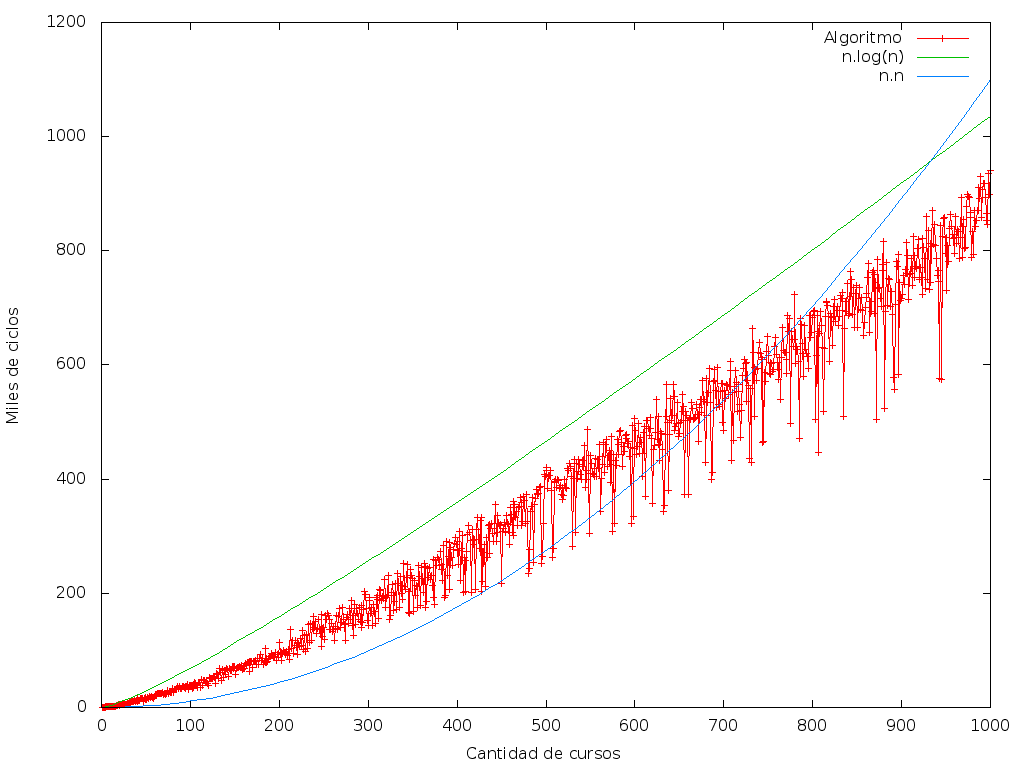
\includegraphics[scale=0.35]{ej2/Graficos/1000casos.png}\\

En el gràfico podemos observar que el algoritmo se encuentra acotado por $n*log(n)$ y es estrictamente menor a $n^2$ lo cual cumple con lo pedido en el enunciado.

